%%
%% This is file `sample-xelatex.tex',
%% generated with the docstrip utility.
%%
%% The original source files were:
%%
%% samples.dtx  (with options: `sigconf')
%% 
%% IMPORTANT NOTICE:
%% 
%% For the copyright see the source file.
%% 
%% Any modified versions of this file must be renamed
%% with new filenames distinct from sample-xelatex.tex.
%% 
%% For distribution of the original source see the terms
%% for copying and modification in the file samples.dtx.
%% 
%% This generated file may be distributed as long as the
%% original source files, as listed above, are part of the
%% same distribution. (The sources need not necessarily be
%% in the same archive or directory.)
%%

\documentclass[sigconf, nonacm]{acmart}

\usepackage{mwe}
\usepackage[colorinlistoftodos,prependcaption,textsize=tiny]{todonotes}


%%
%% \BibTeX command to typeset BibTeX logo in the docs
\AtBeginDocument{%
  \providecommand\BibTeX{{%
    \normalfont B\kern-0.5em{\scshape i\kern-0.25em b}\kern-0.8em\TeX}}}

\begin{document}

%%
%% The "title" command has an optional parameter,
%% allowing the author to define a "short title" to be used in page headers.
\title{Express Data Queueing}

%%
%% The "author" command and its associated commands are used to define
%% the authors and their affiliations.
%% Of note is the shared affiliation of the first two authors, and the
%% "authornote" and "authornotemark" commands
%% used to denote shared contribution to the research.
\author{Freysteinn Alfreðsson}
\email{freysteinn.alfredsson@kau.se}
\orcid{0000-0003-1516-9370}
\affiliation{%
  \institution{Department of Computer Science}
  \city{Karlstad}
  \country{Sweden}
}
\author{Per Hurtig}
\email{per.hurtig@kau.se}
\affiliation{%
  \institution{Department of Computer Science}
  \city{Karlstad}
  \country{Sweden}
}
%%\orcid{0000-0003-1516-9370}
\author{Anna Brunstrom}
\email{anna.brunstrom@kau.se}
\affiliation{%
  \institution{Department of Computer Science}
  \city{Karlstad}
  \country{Sweden}
}

\author{Toke Høiland-Jørgensen}
\email{toke@redhat.com}
\affiliation{%
  \institution{Red hat}
  \country{Denmark}
}

\author{Jesper Dangaard Brouer}
\email{brouer@redhat.com}
\affiliation{%
  \institution{Red hat}
  \country{Denmark}
}

%%
%% By default, the full list of authors will be used in the page
%% headers. Often, this list is too long, and will overlap
%% other information printed in the page headers. This command allows
%% the author to define a more concise list
%% of authors' names for this purpose.
\renewcommand{\shortauthors}{Alfreðsson, et al.}

\begin{abstract}
\end{abstract}

%%
%% Keywords. The author(s) should pick words that accurately describe
%% the work being presented. Separate the keywords with commas.
\keywords{XDP, BPF, BPF, Queueing, Linux, Scheduling}

%%
%% This command processes the author and affiliation and title
%% information and builds the first part of the formatted document.
\maketitle

\section{Introduction}

The Linux kernel is a widely used platform in devices that range from IoT devices, cellphones, home and enterprise routers to servers and cloud offerings. One of the revolutionary technologies of the Linux kernel is the BPF framework, which has changed the way we extend the kernel. This framework is an in-kernel runtime environment that allows domain-specific code to execute within the kernel safely using predefined hooks. One such hook is the Linux eXpress Data Path\cite{hoiland2018express}, or XDP, which introduces a fast data-path within the Linux kernel and has found numerous uses in the industry, such as Denial-of-Service attack mitigation, load-balancers, and intrusion prevention systems.

XDP provides a high-performance programmable network data path and allows programmers to process packets early out of the driver. While XDP excels in forwarding packets, it currently has no mechanism for queuing or reordering of packets and cannot implement traffic scheduling policies. Packet scheduling is a common task on network equipment, and like for other aspects of networking, there is a growing interest for bringing programmability to this domain. For the Linux kernel, making packet scheduling fully programmable through BPF is the obvious answer to this trend.

This paper presents our work on adding programmable packet scheduling to XDP, which we also provide as a Qdisc. We have designed a programmable packet scheduling framework in BPF using recently proposed schemes for programmable queues. This extension allows programmers to define their packet schedulers using BPF while benefiting from the XDP fast data path.


\section{Packet Scheduling, Traffic Shaping, and Queue Management}

Packet schedulers provide the means of controlling the policy and quality requirements within a network for customers and services. However, at its core, the primary function of the packet scheduler is to arrange or rearrange packets to meet the requirements of the network. Most of these requirements are to improve the latency of specific flows or to improve fairness between flows. For instance, video streaming services would like to ensure that clients get fair access to their video streams. Moreover, a service provider might want to prioritize traffic of their productions servers over their testing servers. Therefore, having the flexibility to adapt the packet scheduling algorithm to the requirements of the network in question can significantly improve its overall quality.


\begin{figure}
  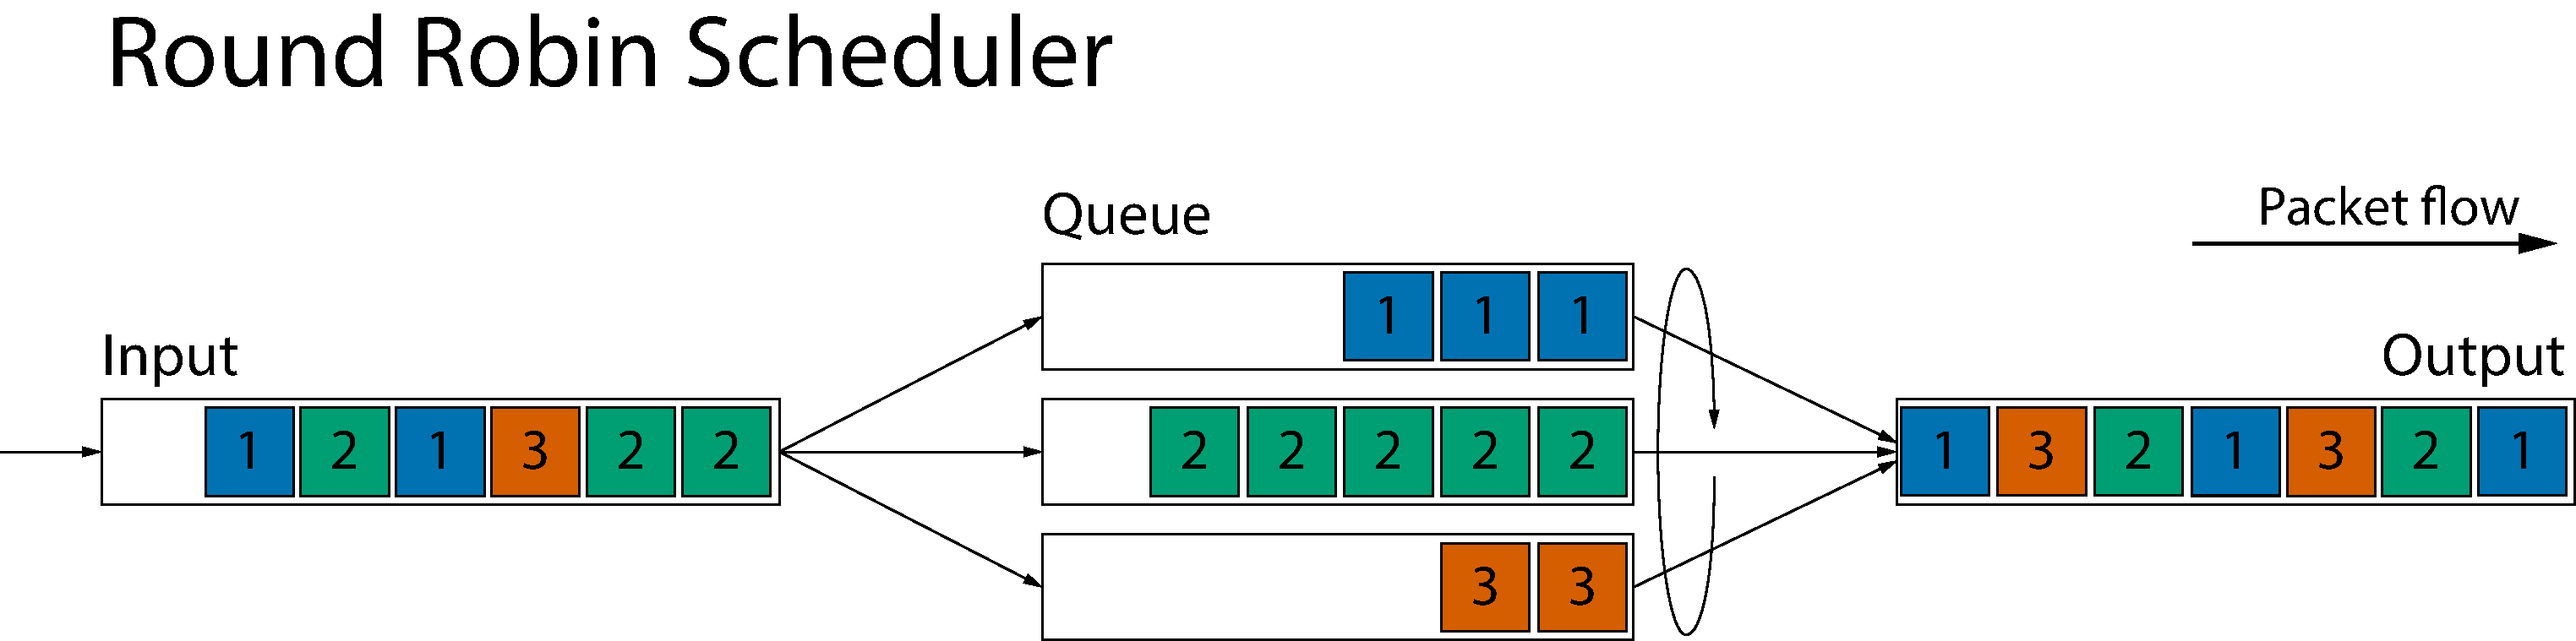
\includegraphics[width=\linewidth]{round-robin.pdf}
  \caption{The Round-Robin scheduler sorts enqueued packets into different queues depending on their flows. On dequeue, the packets are dequeued in a round-robin fashion, giving equal throughput for flows when all packets are equal in size.}
  \label{fig:round_robin}
\end{figure}

A simple example of a packet scheduler is the round-robin scheduler\cite{nagle1987packet}, depicted in Figure~\ref{fig:round_robin}. This scheduler sorts the incoming packets by flow into different queues, which it then dequeues from in a round-robin fashion, or by taking one packet from each queue at the time. This simple scheduler can provide throughput fairness between flows.

%\begin{figure}
%  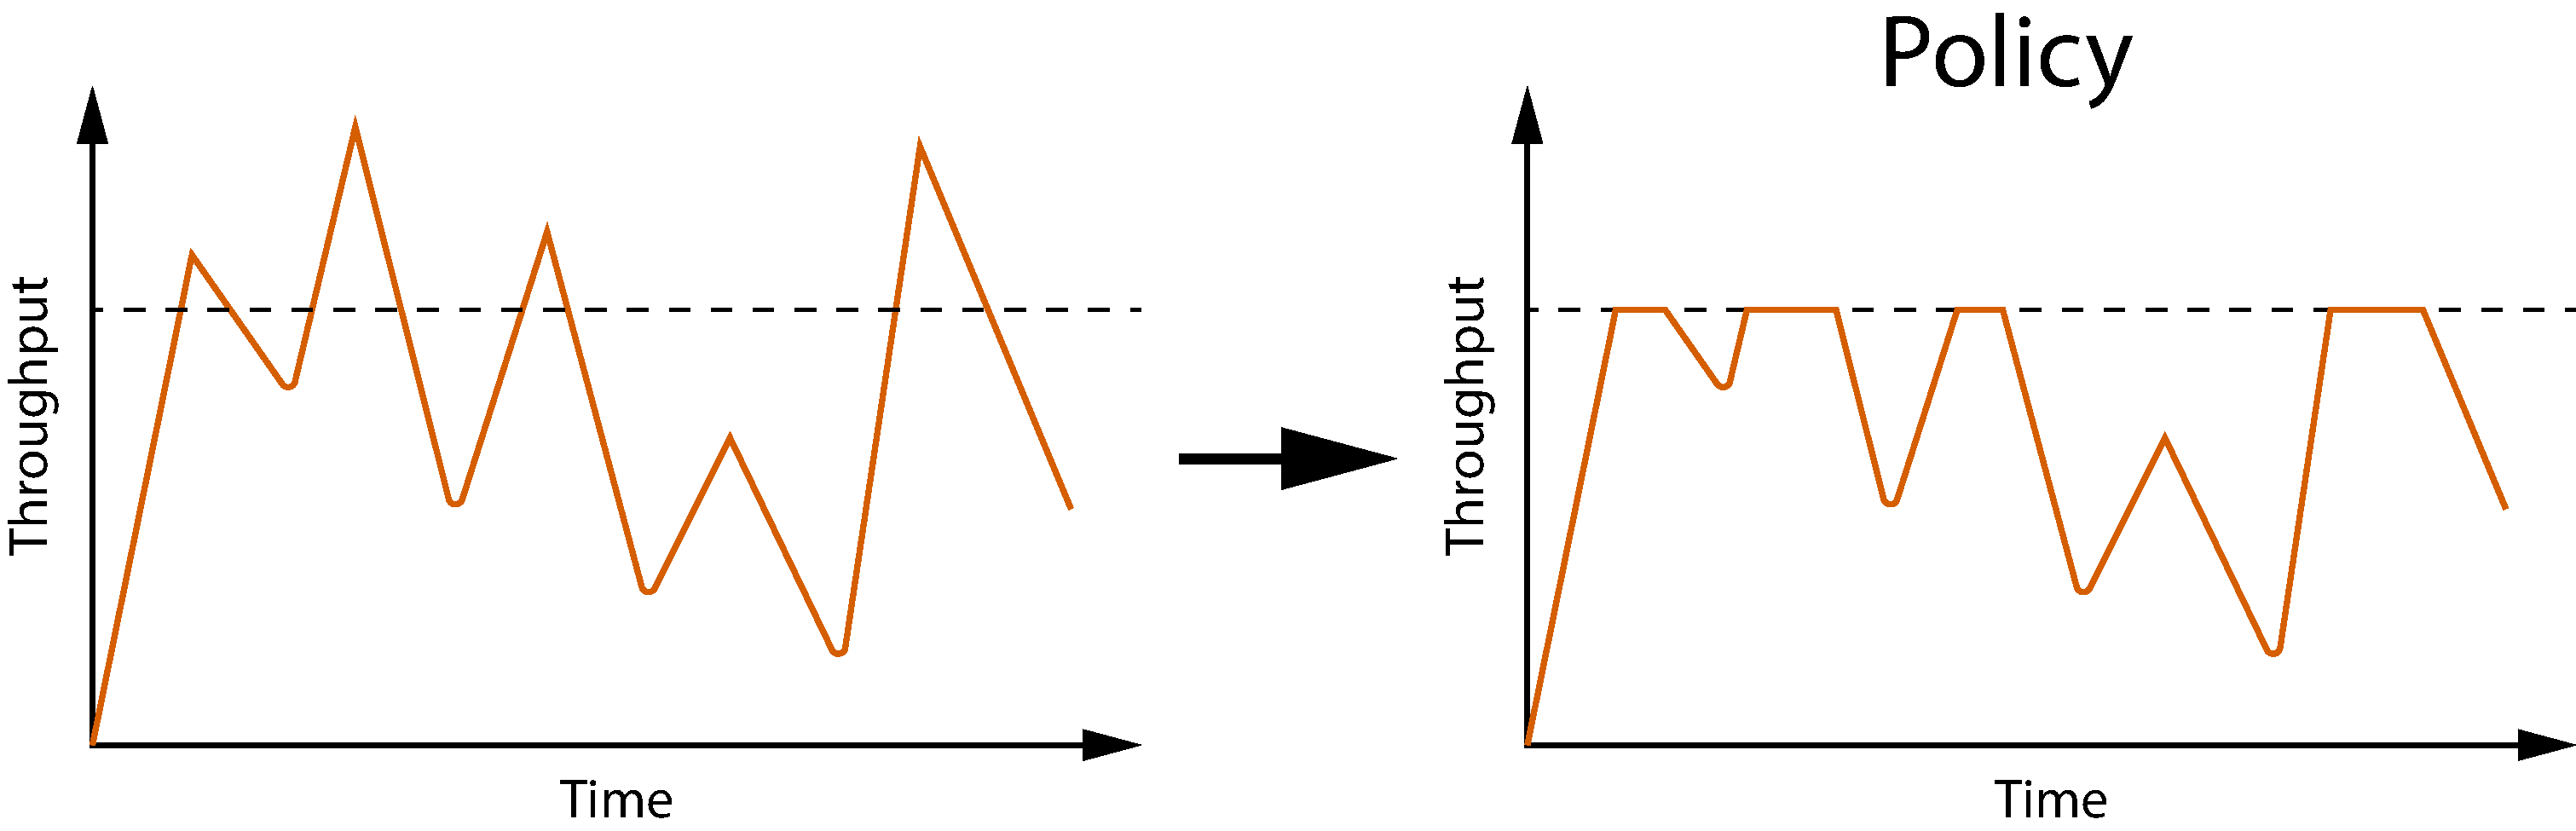
\includegraphics[width=\linewidth]{traffic-policy.pdf}
%  \caption{\label{fig:traffic_policy}}
%\end{figure}

\begin{figure}
  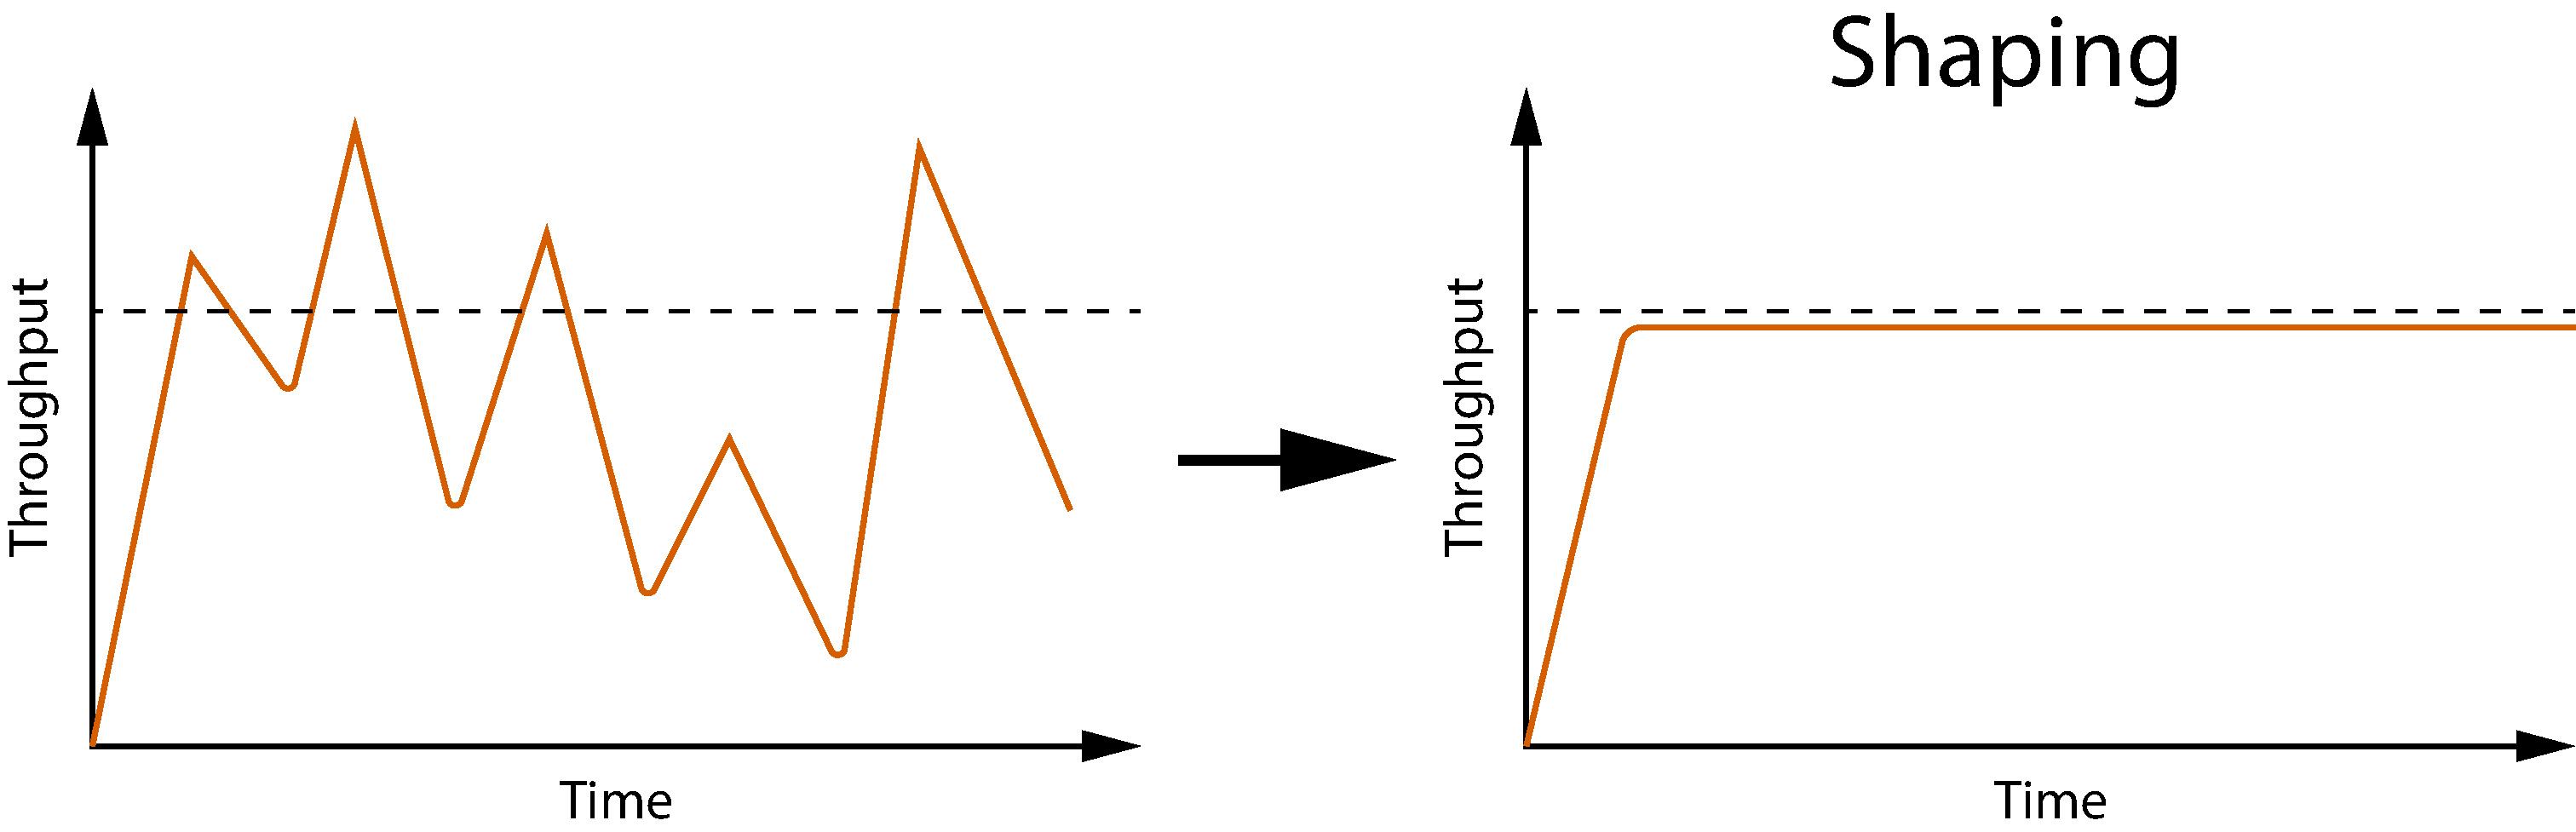
\includegraphics[width=\linewidth]{traffic-shaping.pdf}
  \caption{Traffic shaping is the art of delaying packets to control the throughput. The figure depicts traffic without shaping on the left and the same traffic with shaping on the right.}
  \label{fig:traffic_shaping}
\end{figure}

Another crucial component related to packet schedulers is the capability of delaying packets. This capability allows packet scheduling algorithms to provide traffic shaping, as seen in figure \ref{fig:traffic_shaping}. These algorithms are referred to as non-work conserving algorithms because they do not necessarily use the total capacity of the network interface, while work-conserving algorithms never delay packets and can use their total capacity. An example of a non-work conserving scheduling algorithm would be an ISP enforcing a network policy that guarantees their clients get the bandwidth they promised them.

Queue management is also another essential topic related to packet schedulers and is the art of controlling how many packets the queues can queue. A significant problem in today's environments is bufferbloat, where network vendors have previously favored large buffers for throughput by sacrificing latency. Bufferbloat can negatively affect low latency applications such as video conferencing, online gaming, and other interactive applications. Therefore, queue management is an integral part of the queueing process, while it is not usually considered part of the packet scheduling algorithm.


\section{The Linux Kernel Networking Subsystem}

\begin{figure}
  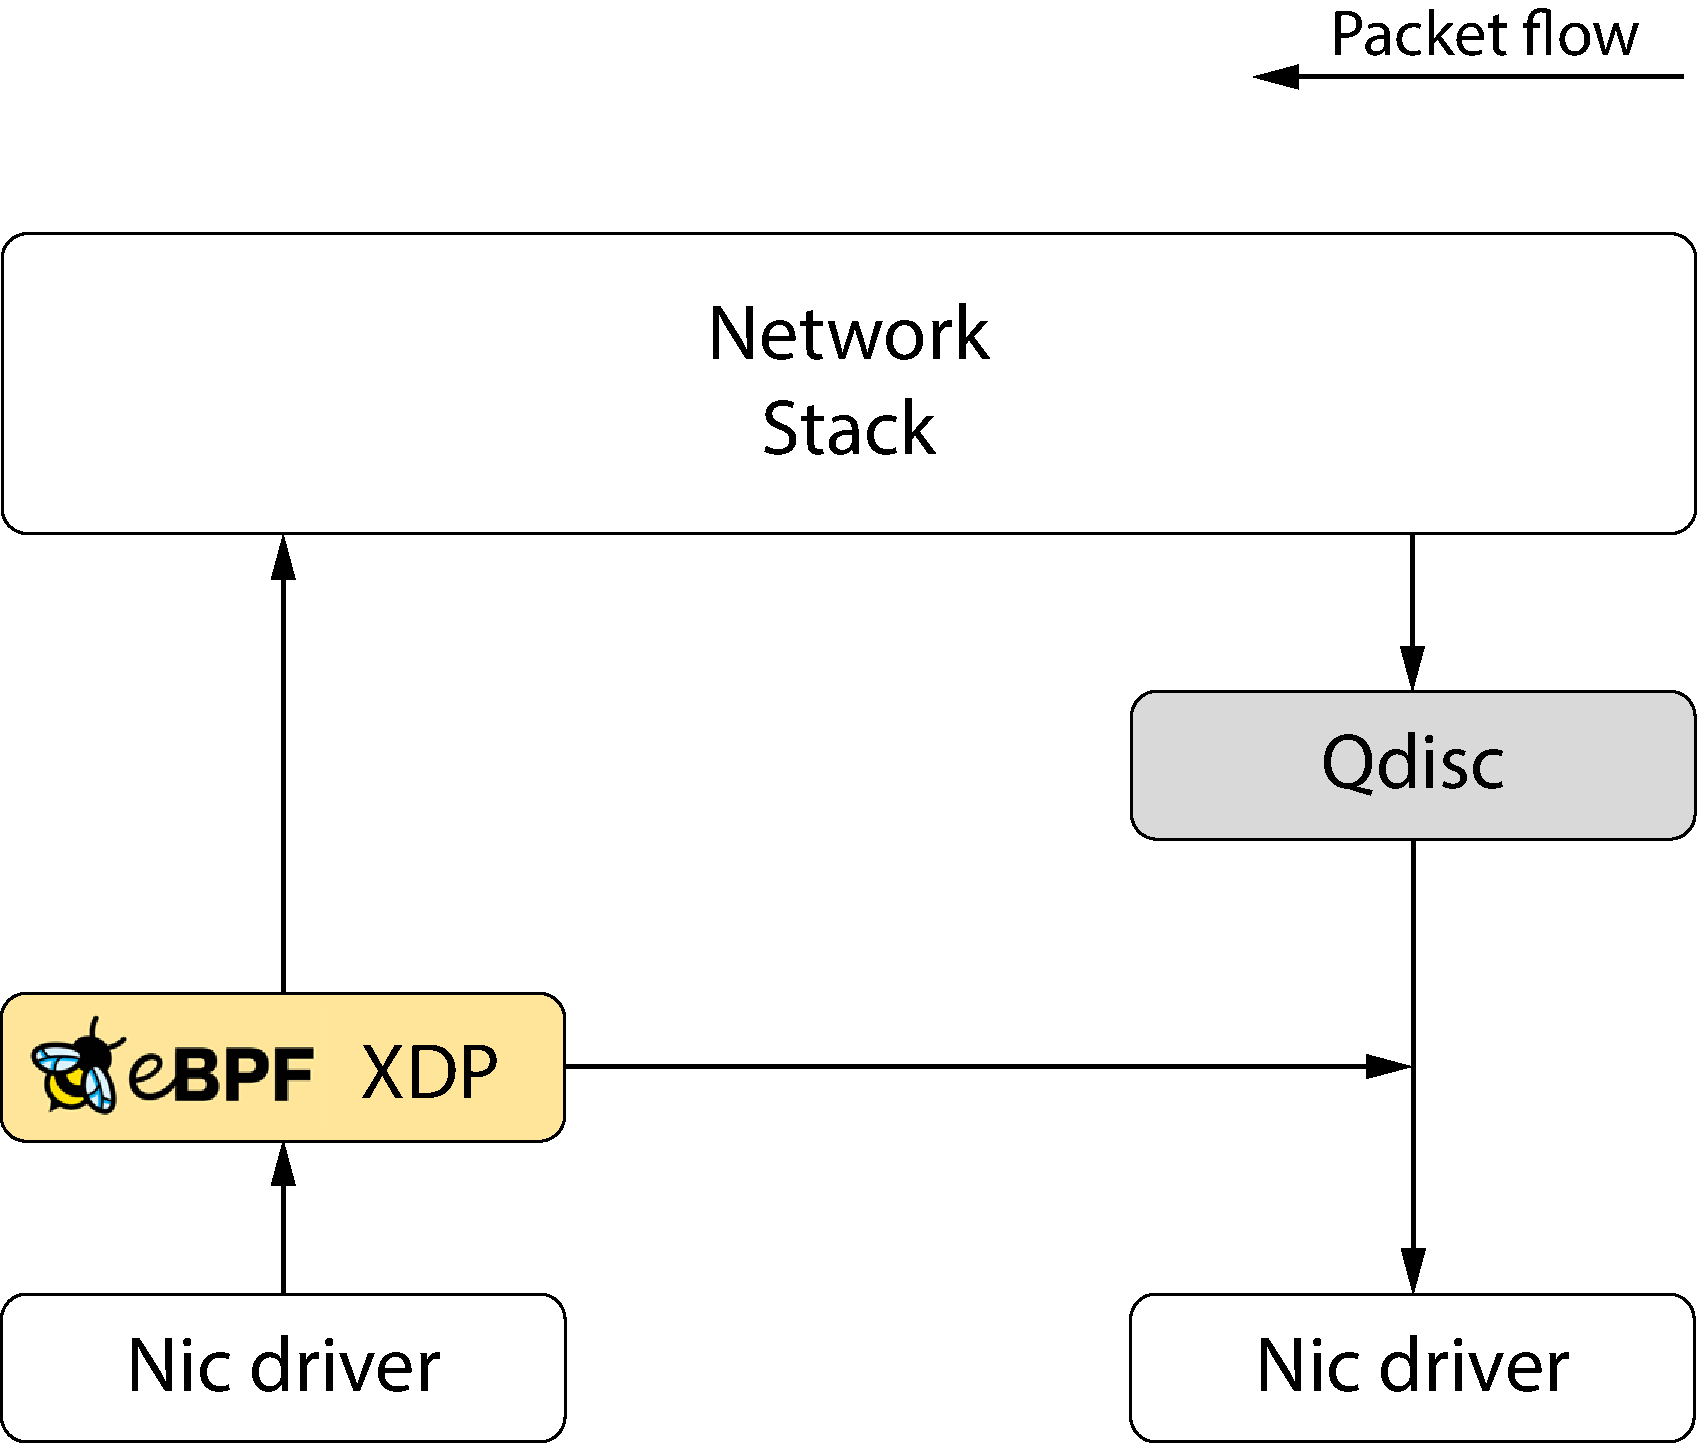
\includegraphics[width=0.6\linewidth]{network-overview.pdf}
  \caption{XDP allows network application programmers to write code that runs on every network packet using the BPF framework. XDP gives the programmer the capability to modify the packet and redirect the packet using the code's return value. The possible return values are as follows: 1) Passing the packet to the kernel's networking stack. 2) Redirecting the packet to another network device. 3) Send the packet directly out on the same device. 4) Or dropping the packet altogether.}
  \label{fig:network_overview}
\end{figure}

The Linux kernel Networking stack is highly mature and a flexible piece of software. It contains a hardware abstraction layer, a traffic control layer responsible for routing and firewall rules, and layers responsible for handling the TCP/IP networking layers. Part of the traffic control layer is the Queueing discipline layer or the Qdisc layer for short. This layer gives the Linux kernel flexible packet scheduling capabilities and an interface to create new packet schedulers as loadable kernel modules. However, due to the immense speed increases in modern network devices, the kernel's networking stack has become a bottleneck. This obstacle has prompted network vendors and researchers to create alternative solutions to mitigate this performance bottleneck. One such solution is DPDK which bypasses the Linux kernel and communicates directly to the networking hardware. An alternative solution to bypassing the Linux kernel, which we describe in section~\ref{sec:xdp}, is XDP, which creates a fast data path within the Linux kernel while retaining the kernel and user-space separation. We provide a simplified diagram of the Linux kernel's networking infrastructure in Figure \ref{fig:network_overview} which shows the relevant parts related to our work in this paper. It shows how XDP can steer traffic either through the network stack or bypass it altogether.

% Frey: The idea of this paragraph was to prepare a bit of differences between the BPF queuing implementation between the Qdisc and XDP. However, I am commenting this section out until we have more implementation information and see how relevant this section is at that point.
% The primary networking data structure in the Linux kernel is the sk\_buff. The sk\_buff is a large data structure with multiple fields related to all layers in the network stack and gets populated through each layer of the network stack, including the Qdisc layer. However, XDP handles network packets in the driver right after a DMA synchronization. Therefore, it does not use the sk\_buff data structure but represents the packet using a slimmer data structure called xdp\_frame, which does not get converted into a sk\_buff unless the XDP hook passes the packet onto the network stack.


\subsection{The Linux Kernel Packet Queueing Discipline (Qdisc)}

Packet scheduling in the Linux kernel is handled by the Qdisc subsystem. It is a mature system that is capable of wast operations, such as policing, shaping, classifying, dropping, and marking traffic.

\begin{itemize}
  \item Explain where in the network pipe the Qdiscs are located.
  \item Explain that the Qdisc layer allows us to create hierarchies of preexisting Qdiscs.
  \item Explain what the Qdisc classifier does.
  \item Explain what the BPF Qdisc classifier does and why it does not fulfill our needs.
\end{itemize}


%\section{Packet Schedulers in Practice}
%
%\todo[inline]{Frey: This section needs a new name. The idea with this section is to explain why we care about this work and what the requirements are.}
%
%\begin{itemize}
%  \item Explain what is not possible using today's packet schedulers.
%  \item Explain why you would like to be able to schedule traffic
%\end{itemize}


\section{Programmable Packet Schedulers}

\begin{figure}
  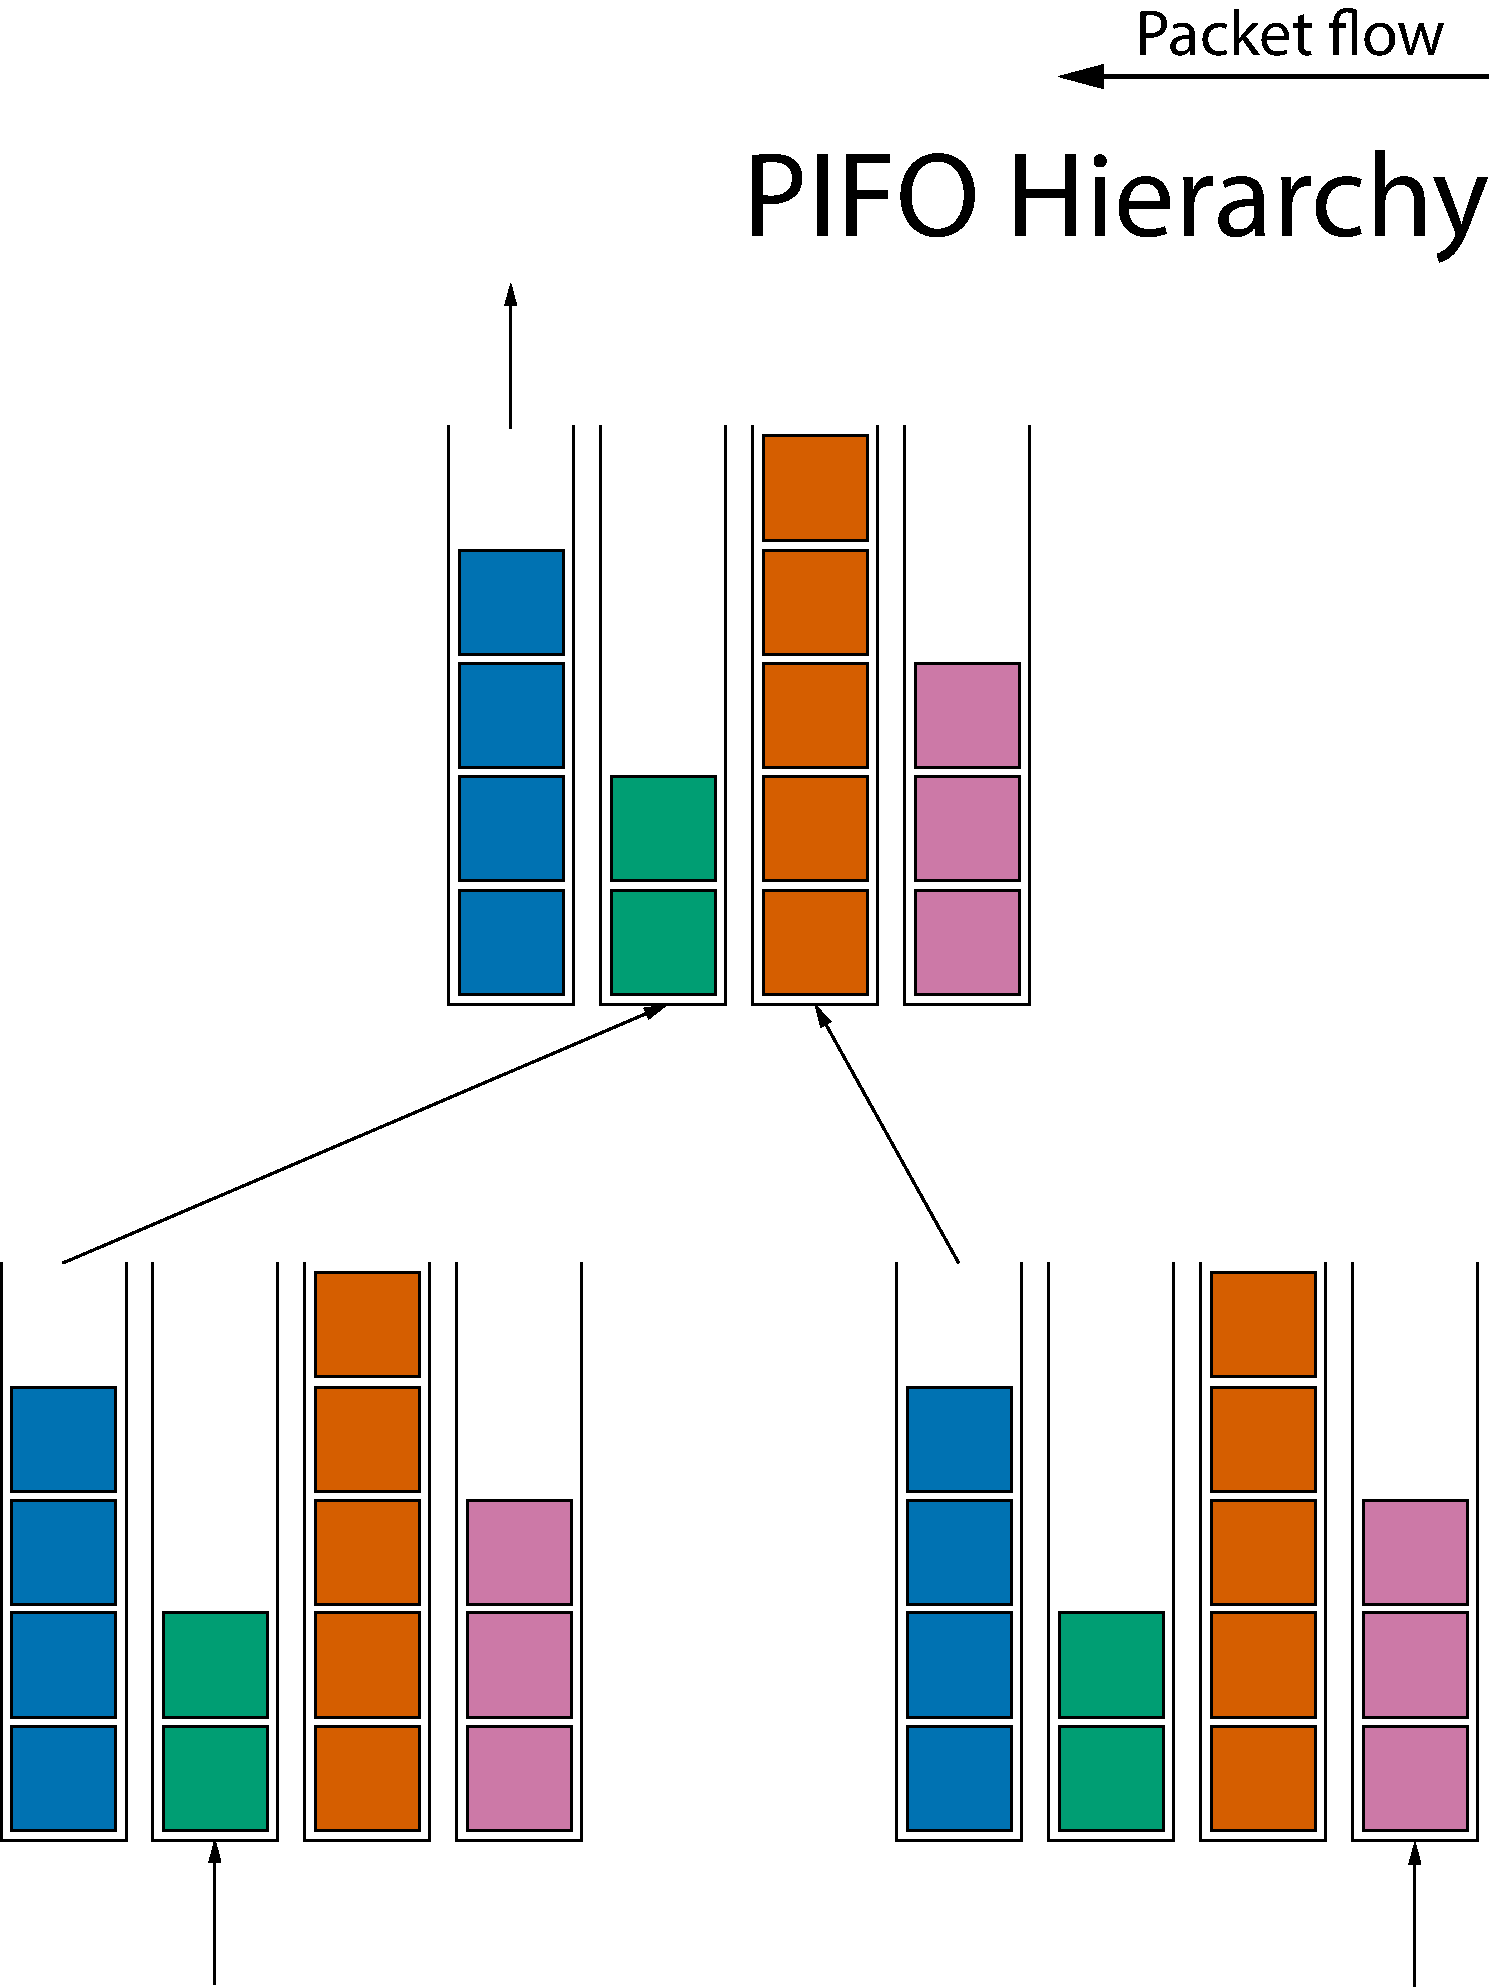
\includegraphics[width=0.5\linewidth]{pifo-hierarchy.pdf}
  \caption{We can implement complex packet scheduling algorithms by forming hierarchies of PIFO and the Eiffel data structures. Some packet schedulers need hierarchies to function. However, we can also use hierarchies to combine different schedulers to handle complex requirements.}
  \label{fig:pifo_hierarchy}
\end{figure}

Traditionally, network equipment and operating systems provide a handful of packet scheduling algorithms. This limited number of schedulers forced companies to tune the parameters of these algorithms to meet their requirements. However, modern networking equipment has started to provide programmable network capabilities, which the network engineer can leverage using specialized programming languages such as P4\cite{p4} or standard programming languages such as C, such as in the case of traditional operating systems. This new offering allows the network designers to create custom logic and custom packet scheduling solutions optimized for their specific unique use case. Therefore, instead of tuning the network to the limitations of the packet scheduling algorithm, they can tune their packet scheduling algorithm directly to their network requirements.

Consequently, the building blocks of a programmable packet scheduling framework need to be straightforward, fast, and easy to understand. Therefore, the essential part of creating a programmable packet scheduling framework is to provide a flexible data structure. Therefore, this has become an active research area to develop a flexible data structure that programmers can leverage to implement their packet schedulers. However, due to the vast speeds of modern network interfaces, severe time limitations are put on these data structures, which tend to make generic priority queues, such as red-black trees and binary heaps, unsuitable choices.

In this paper, we focus on the two priority queues, PIFO and Eiffel, described in sections~\ref{sec:pifo} and \ref{sec:eiffel}. Both are simple data structures that share the following qualities. They use an integer-based ranking function to queue packets by their priority and rely on a fixed range of ranks known at initialization time. They dequeue according to the scheduled packet order. Furthermore, they both have the flexibility to create complex packet scheduling algorithms by using hierarchies, as seen in Figure~\ref{fig:pifo_hierarchy}. However, Eiffel differs in that it can make scheduling decisions on dequeue, while PIFO only makes scheduling decisions on enqueue. This distinction stems from the fact that PIFOs are well suited for both hardware and software. However, Eiffel is a software-only data structure and is, therefore, capable of more complex operations, such as flow-based scheduling, which requires scheduling on dequeue.


\subsection{PIFO and SP-PIFO} \label{sec:pifo}

Despite its simplicity, the Push-In First-Out data structure\cite{Sivaraman2016} is quite versatile and allows the programmer to implement a wide range of packet schedulers. From a programmer's perspective, the programmer only needs to decide what order to schedule packets and when to schedule them for non-work conserving algorithms. However, one limitation of the PIFO is that each FIFO, and therefore, each rank takes memory. Therefore, the more granularity of ranks, the more resources the PIFO needs. This limitation limits how large the PIFO can be both in hardware and software implementations. A mitigation to this limitation is the SP-PIFO\cite{Alcoz2020}, which approximates a large PIFO using a smaller PIFO.

\begin{figure}
  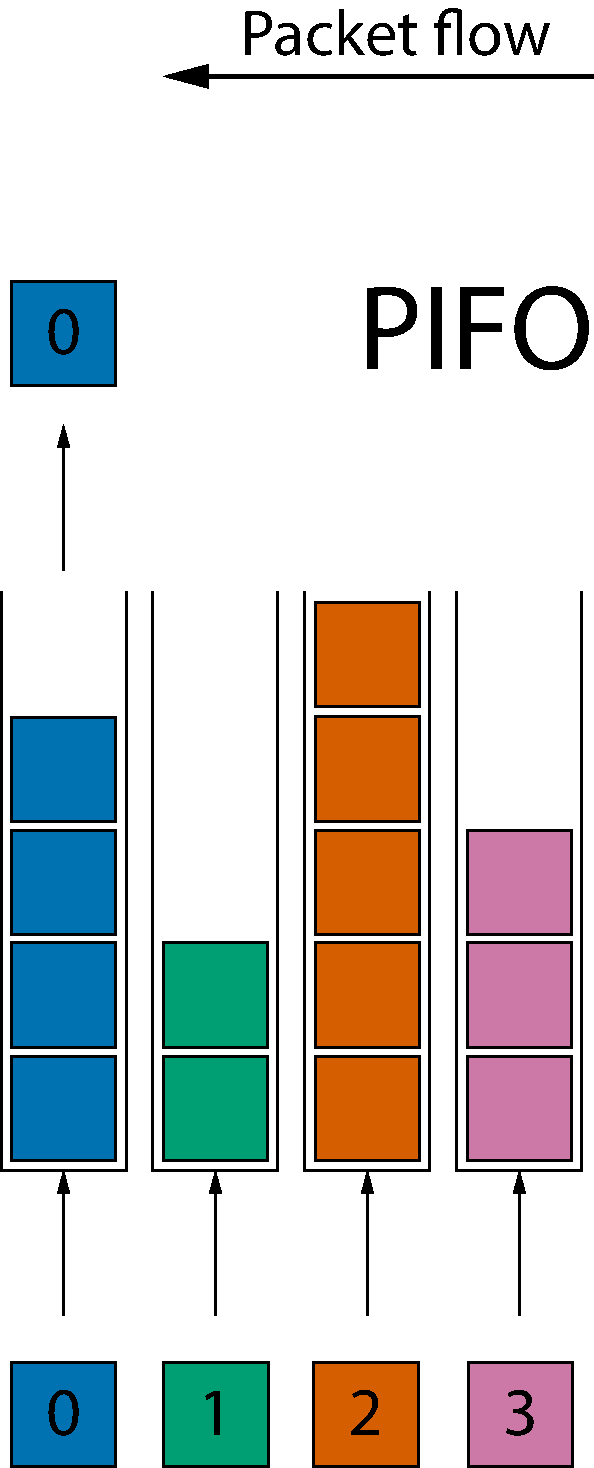
\includegraphics[width=0.25\linewidth]{pifo.pdf}
  \caption{\todo[inline]{I think we should discuss better ways to draw both the PIFO and Eiffel data structures. I think it might be better to have two different pictures—one for PIFO and another for Eiffel with references to queues.}}
  \label{fig:pifo}
\end{figure}

\subsubsection{Data Structure}

The PIFO is a priority queue where the programmer can queue packets based on their rank, where each rank is queued in a FIFO order, as shown in Figure~\ref{fig:pifo}. However, the programmer can only dequeue from the head of the PIFO and only order packets on enqueue. However, the PIFO does not allow reordering the packets within a FIFO. Nor can it reorder the packets on deqeue. This limitation does exclude the PIFO from implementing some packet scheduling algorithms, such as pFabric\cite{alizadeh2013pfabric}.


\subsection{Eiffel} \label{sec:eiffel}

The Eiffel data structure is an efficient software implementation of a PIFO with a couple of alterations. First, in Eiffel, the programmer can schedule flows or packets, depending on the algorithm, where each flow is a separate FIFO that contains only the flow's packets. The Eiffel data structure can schedule references to those FIFOs instead of the individual packets. Second, the programmer can do on-dequeue scheduling; this allows the algorithm to virtually rearrange all the packets from the same flow by simply requeueing the reference to that flow back into the Eiffel data structure. These two additions allow the Eiffel data structure to represent more scheduling algorithms than PIFO, such as pFabric\cite{alizadeh2013pfabric}.

Also, because Eiffel is a software implementation, the Eiffel paper proposes a few software-based optimizations to improve the performance of the Eiffel data structure. One such optimization is to use a bit-field to keep track of queues containing packets and use the CPUs Find-First-Set instruction to accelerate the lookup in the bit lookup table. The lookup table can be further segmented into a tree-based lookup table when the Eiffel has many ranks.


\section{The BPF framework}

The BPF framework is an in-kernel runtime environment that allows specialized programs to execute in the kernel safely. These programs attach themselves to hooks provided by the different subsystems of the kernel. These hooks limit what the programs can do and define what type of BPF programs can exist. These types of programs vary but predominantly, they are related to networking, tracing, and security. From a user-space perspective, BPF represents the program code as a specialized BPF instruction set. However, as a framework, it provides an execution environment, a key-value store for inter-process communication called BPF maps, in-kernel helper functions, and toolchains to create and manage BPF programs from user-space.

\begin{itemize}
  \item Explain BPF maps and their scope.
  \item Explain what hooks are and that BPF allows helper functions.
\end{itemize}


\subsection{Express Data Path (XDP)} \label{sec:xdp}

XDP\cite{hoiland2018express} is a type of BPF program that is attached directly to the RX path of a network interface to allow the programmer direct manipulation of packets from the network driver. Its primary use cases are high-performance packet processing and the ability to bypass the kernel's network stack by redirecting the packet to different locations, such as back out the same device, to another device, or dropping the packet entirely. XDP also provides helper functions that allow the programmer to call particular parts of the network stack, such as fib lookups.

While XDP excels at forwarding packets, it does not support packet reordering or packet scheduling. Our objective in this paper is to extend XDP to support packet scheduling. This support includes adding helper functions and extra hooks for dequeuing and pacing operations.


\subsection{BPF Qdisc Classifiers}

Currently, the Qdisc layer only has a BPF classifier capable of manipulating packets and directing them into excising Qdiscs that are not programmable using BPF. While this does provide a form of programable packet scheduling, it relies exclusively on the Qdisc layer, which XDP can not use. We aim to provide a BPF based packet scheduling framework for XDP and as a standalone Qdisc.


\section{A Programmable Packet Scheduling Framework in BPF}

\begin{figure}

  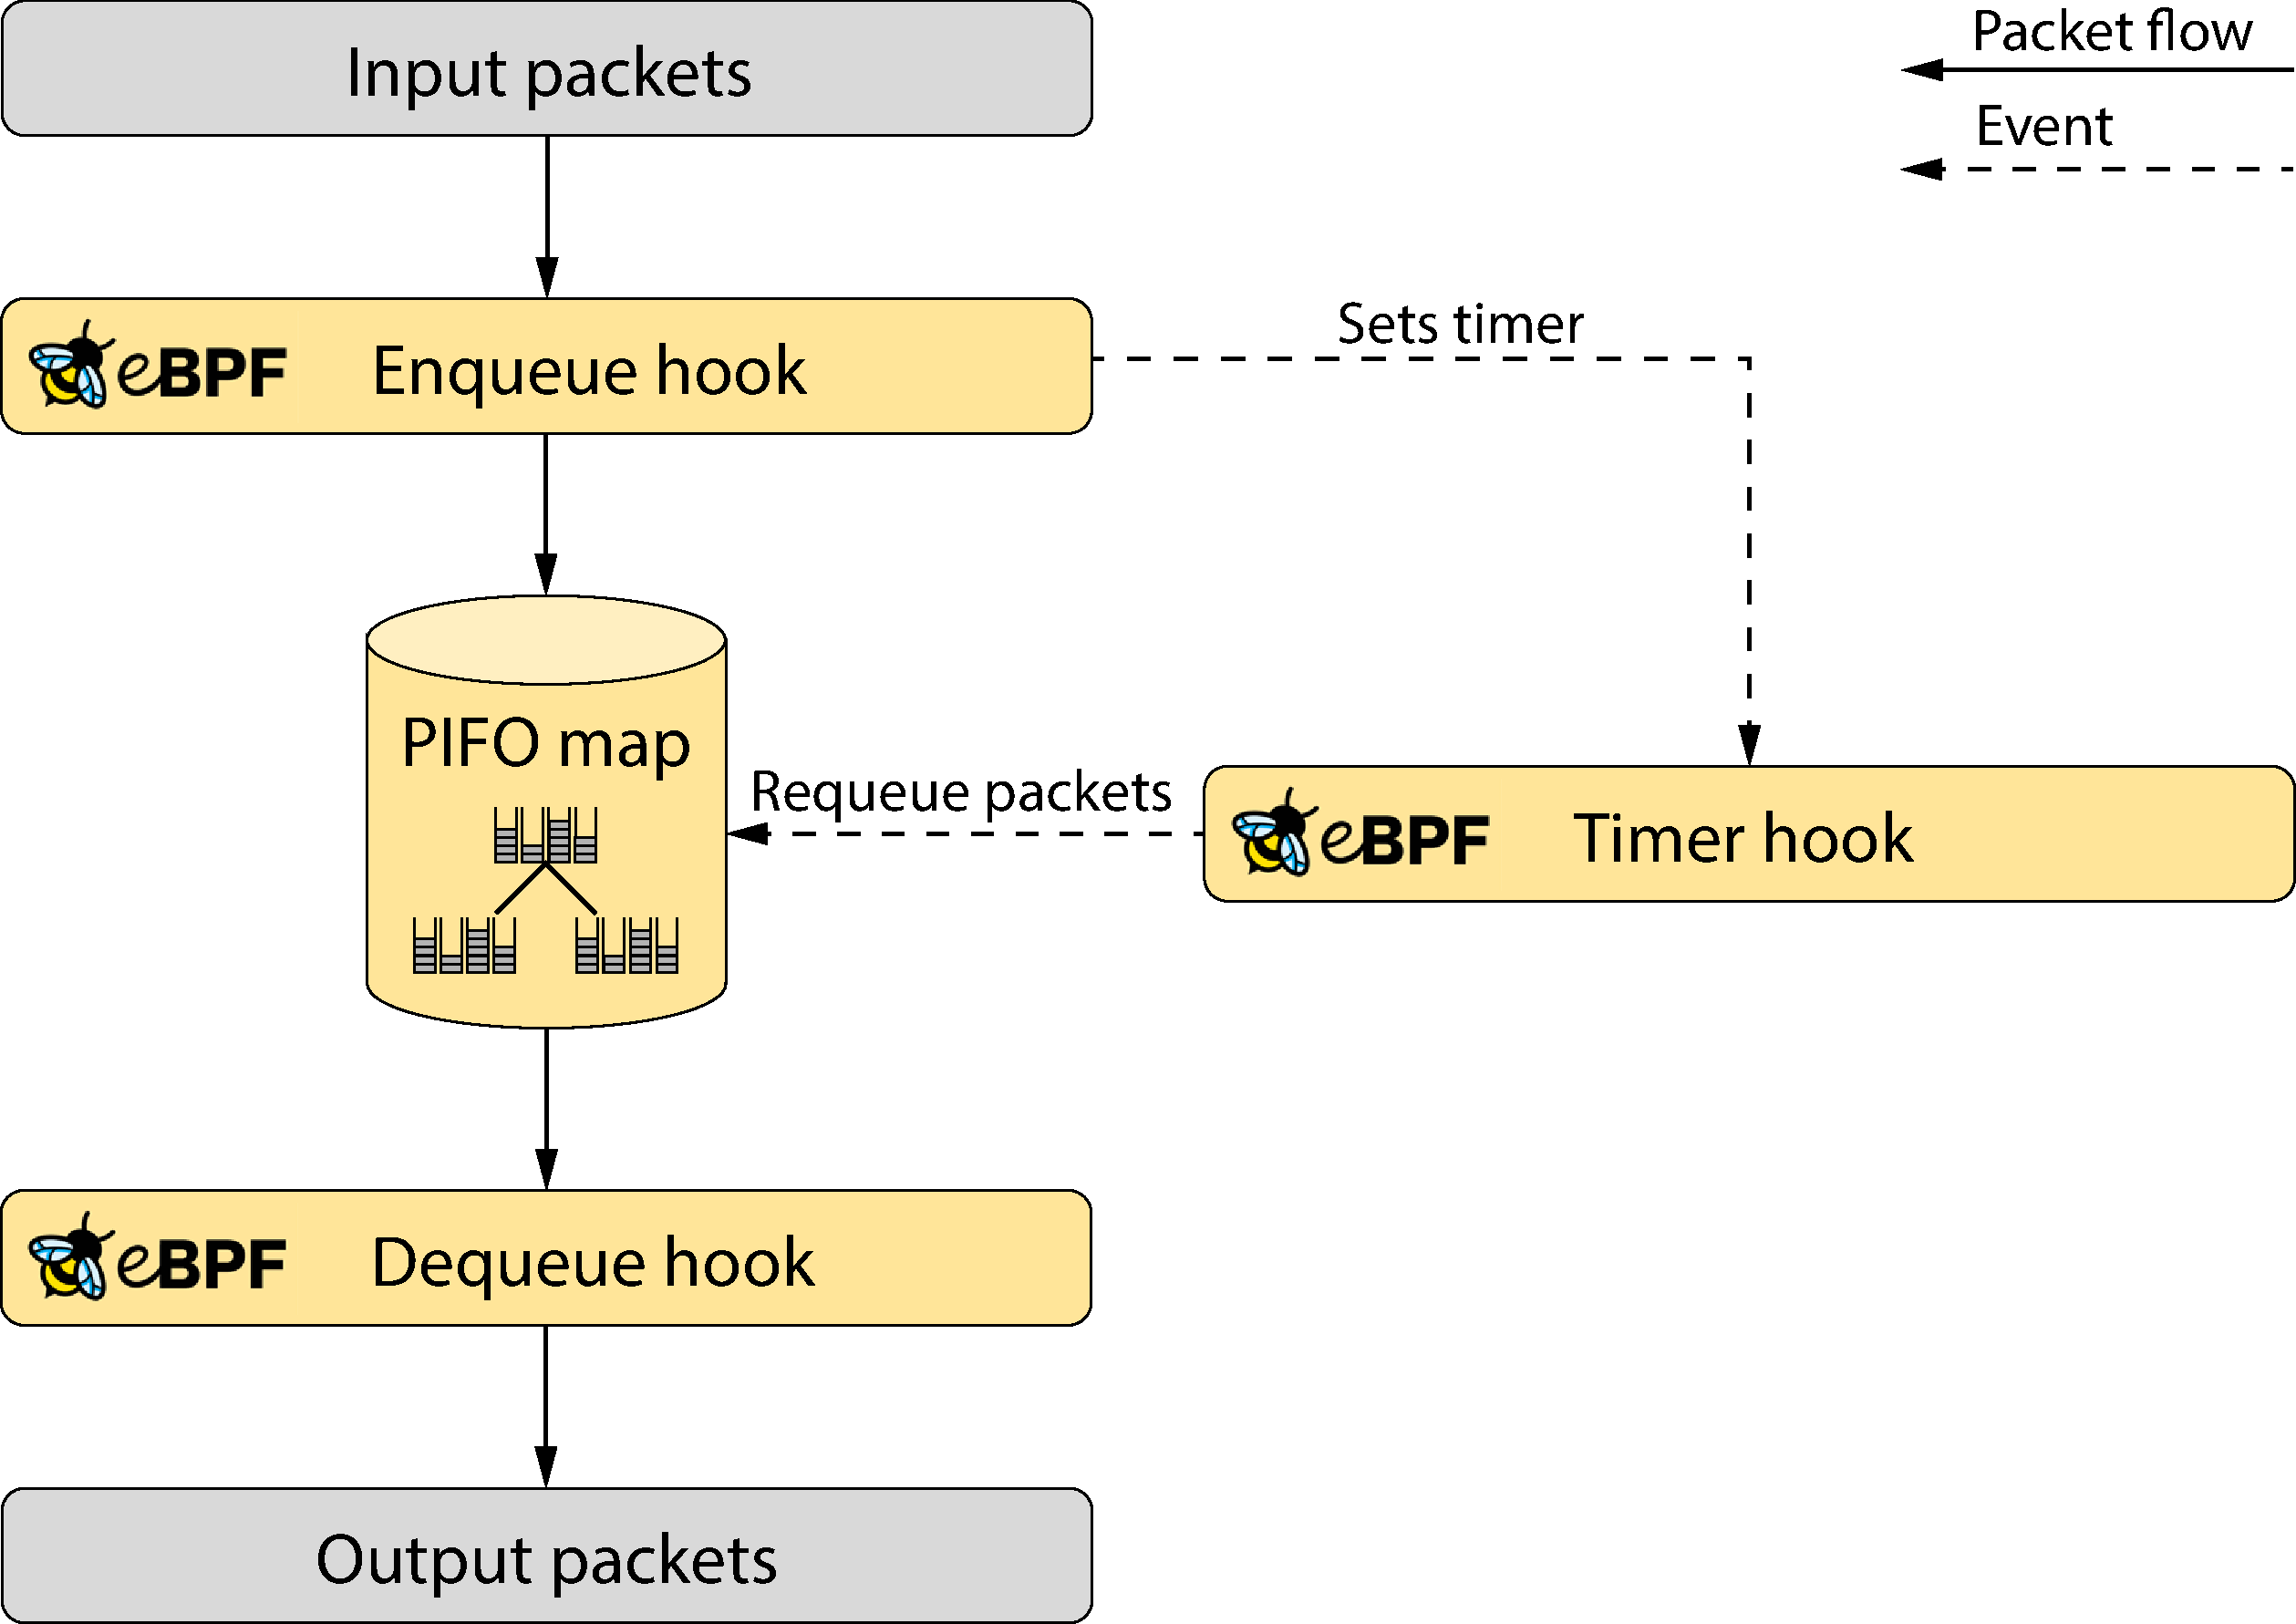
\includegraphics[width=\linewidth]{bpf_pps_flow.pdf}

  \caption{Depicted are the BPF hooks needed to implement programmable packet scheduling using our framework. The main hooks are the enqueue and dequeue hooks, with the optional timer hook. Queueing works the same in both XDP and the Qdisc. However, they do not use the same enqueue and dequeue hooks.}
  \label{fig:bpf_pps_flow}
\end{figure}

We have created an BPF based programmable packet scheduling framework that is flexible enough to share between the XDP and kernel Qdisc layers. The design is depicted in Figure \ref{fig:bpf_pps_flow}, which shows the basic building blocks for our design without the specifics of XDP nor the Qdisc subsystem.

These building blocks are then further broken down as follows:

\begin{itemize}
        \item Queue map: This new BPF map implements a PIFO and is the main building block for the programmer to create packet schedulers.
        \item Enqueue hook: This BPF hook is responsible for redirecting packets to BPF queue maps. This is the standard XDP hook in the case of XDP. However, it is a new hook in Qdiscs.
        \item Timer hook: This is an optional hook and is only required for algorithms that delay packets, e.g., packet pacing or traffic shaping. It is responsible for dequeuing and enqueuing packets from different PIFOs to introduce delayed packets. We implement timers using the newly introduced BPF timer API. This API allows the programmer to schedule BPF programs to be run at a specified time in the future, which can be used to release held packets.
        \item Dequeue hook: This hook is responsible for delivering the packet from the packet scheduling algorithm. In XDP, this is a new hook that each driver calls to transmit a packet. It can deliver bulking by repeatedly calling the hook to dequeue multiple packets before it transmits them.
\end{itemize}

Our design represents the PIFO data structure as an eBPF map. This representation allows the BPF programs to use a familiar map interface to reference PIFOs straightforwardly in their scheduling algorithm. From a programmer's perspective, the eBPF hooks reference the queues like any other map type. The enqueue hook decides which queue to direct the packet to by a map reference. Similarly, the dequeue hook picks which queue map to dequeue from and returns a reference to the dequeued packet to the kernel for transmission. For shaping scheduling algorithms, the BPF packet scheduling hooks set BPF timers that trigger BPF programs at specified times. The BPF timer API supports nanosecond precision using the kernel's \textit{hrtimers}, making it ideal for our use case.


\section{BPF-Qdisc}

\todo[inline]{Frey: I am leaving this section here for now. My original idea was that this section would detail how we implemented queueing in XDP. This could include what drivers were changed and where in the pipeline we did the changes.}

To support our new queueing API both for forwarded packets and through locally generated traffic, we provide a separate BPF-Qdisc. This Qdisc still relies on the Linux kernel and does not use XDP. While it does not use the same hooks as XDP, it allows the packet scheduling programmer to use the same queueing API.


\section{XDP Queueuing}

\todo[inline]{Frey: I am leaving this section here for now. My original idea was that this section would detail how we implemented queueing in XDP. This could include what drivers were changed and where in the pipeline we did the changes.}

Our design extends XDP by adding a new dequeue hook into the network drivers. We rely on standard XDP to enqueue packets into BPF queue maps. However, the new dequeue hook supports bulking by having the driver repeatedly dequeue packets from the dequeue hook before it transmits the packets.


\section{Evaluation of BPF-Qdisc and XDP Queueing}

\begin{itemize}
  \item Compare a type of scheduling algorithm using BPF-Qdisc and XDP Queueing performance to Qdiscs that does the same functionality.
  \item Compare BPF-Qdisc and XDP Queueing performance.
\end{itemize}

\section{Conclusion}

\begin{itemize}
  \item Reiterate main points of design, and summarize results.
\end{itemize}



\bibliographystyle{ACM-Reference-Format}
\bibliography{references}


\end{document}
\endinput
